\documentclass{standalone}
\usepackage{tikz}
\usetikzlibrary{positioning,circuits.ee.IEC}

\begin{document}
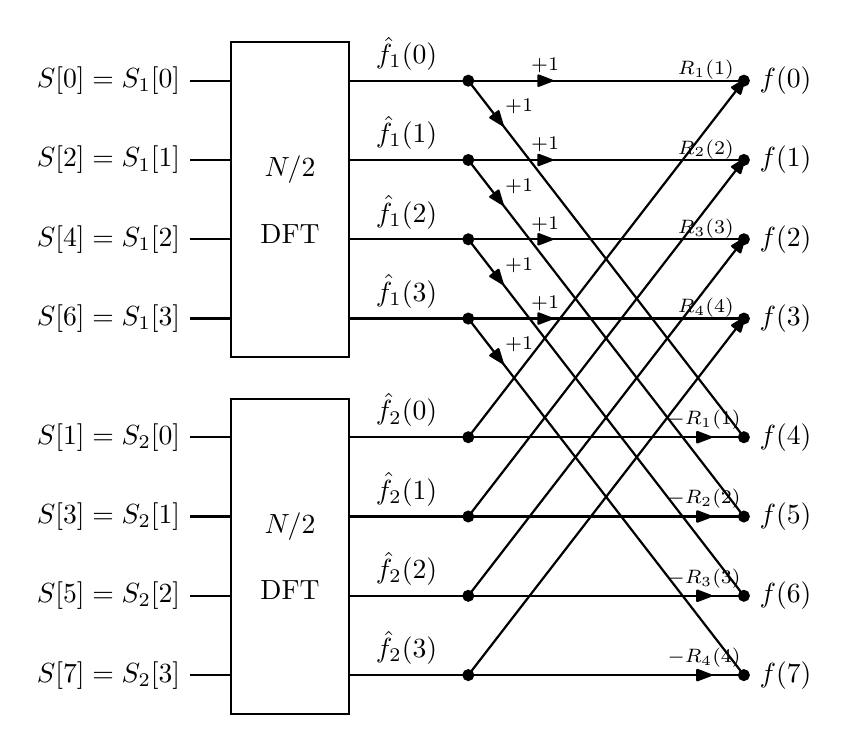
\begin{tikzpicture}
% Style
[
    thick, node distance=.5cm, circuit ee IEC,
    box/.style={
        draw, align=center, shape=rectangle, minimum width=1.5cm, minimum height=4cm,
        append after command={% see also: https://tex.stackexchange.com/a/129668
            \foreach \side in {east,west} {
                \foreach \i in {1,...,#1} {
                %  oordinate (\tikzlastnode-\i-\side)
                %  at ($(\tikzlastnode.north \side)!{(\i-.5)/(#1)}!(\tikzlastnode.south \side)$)
                    (\tikzlastnode.north \side) edge[draw=none, line to]
                        coordinate[pos=(\i-.5)/(#1)] (\tikzlastnode-\i-\side) (\tikzlastnode.south \side)
                }
            }
        }
    }
]

%=================================== Start ===================================
{
    \node[box=4] (box-t) {$N/2$ \\\\ DFT};
    \node[box=4, below=of box-t] (box-b) {$N/2$ \\\\ DFT};

    \foreach \s[count=\i] [
        evaluate={\sa=int(\s*2)},
        evaluate={\sb=int(\s*2+1)}
    ] in {0,1,2,3} {
        \path (box-t-\i-west) edge node[at end, left]{$S[{\sa}] = S_1[\s]$} ++(left:.5);
        \path (box-b-\i-west) edge node[at end, left]{$S[{\sb}] = S_2[\s]$} ++(left:.5);
    }
    \foreach \b/\s[count=\k] in {t/1, b/2} {
        \foreach \i [
            evaluate={\j=int(\i-1)},
            evaluate={\J=int(ifthenelse(\k==2,\j+4,\j))}
        ] in {1,...,4} {
            \node [contact] (conn-\b-\i) at ([shift=(right:1.5)] box-\b-\i-east) {}
            edge node[above] {$\hat{f}_{\s}(\j)$} (box-\b-\i-east)
            node [contact, label=right:{$f(\J)$}] (conn-\b-\i') at ([shift=(right:5)] box-\b-\i-east) {};
        }
    }  

    \begin{scope}[every info/.append style={font=\scriptsize, inner sep=+.5pt}]
    {
        \foreach \i [
            evaluate={\j=int(\i-1)},
            evaluate={\J=int(\i+3)}
        ] in {1,...,4} {
            \path (conn-t-\i) edge[current direction={pos=.27 , info=$+1$           }] (conn-t-\i');
            \path (conn-t-\i) edge[current direction={pos=.1  , info=$+1$           }] (conn-b-\i');
            \path (conn-b-\i) edge[current direction={pos=.87 , info={$-R_{\i}(\i)$}}] (conn-b-\i');
            \path (conn-b-\i) edge[current direction={pos=.999, info={$ R_{\i}(\i)$}}] (conn-t-\i');
        }
    }
    \end{scope}
}
%==================================== END ====================================

\end{tikzpicture}
\end{document}